\documentclass[a4paper, 12pt]{article}
\usepackage[left=2.5cm, right=2.5cm, top=3cm, bottom=3cm]{geometry}
\usepackage[spanish]{babel}
\usepackage{amsmath}
\usepackage{graphicx}
\usepackage{color}
\usepackage{xcolor}
\usepackage[utf8]{inputenc}
\usepackage[T1]{fontenc}
\usepackage{listings}




\definecolor{colorgreen}{rgb}{0,0.6,0}
\definecolor{colorgray}{rgb}{0.5,0.5,0.5}
\definecolor{colorpurple}{rgb}{0.58,0,0.82}
\definecolor{colorback}{RGB}{255,255,204}
%Definiendo el estilo de las porciones de codigo
\lstset{
 backgroundcolor=\color{colorback},
commentstyle=\color{colorgreen},
keywordstyle=\color{colorpurple},
numberstyle=\tiny\color{colorgray},
stringstyle=\color{colorpurple},
basicstyle=\ttfamily\footnotesize,
breakatwhitespace=false,
breaklines=true,
captionpos=b,
keepspaces=true,
numbers=left,
showspaces=false,
showstringspaces=false,
showtabs=false,
tabsize=2,
frame=single,
framesep=2pt,
rulecolor=\color{black},
framerule=1pt
}



\begin{document}


\begin{center}
\text{\Huge Moogle!}\\
\vspace {2cm}
\text{\huge Richard Alejandro Matos Arderí C111}\\
\vspace {1cm}
\text{\Large Facultad de Matemática y Computación, Universidad de La Habana}\\
\vspace {0.5cm}
\text{2023}\\
\vspace {10cm}
\begin{figure}[h]
       \center
       
\includegraphics[width=8cm]{matcom.jpg}
\end{figure}
\end{center}

\newpage
\begin{abstract}
Moogle! es una aplicación  cuyo propósito es buscar inteligentemente un texto en un conjunto de documentos. Es una aplicación web, desarrollada con tecnología .NET Core 6.0, específicamente usando Blazor como *framework* web para la interfaz gráfica, y en el lenguaje C\#.
\end{abstract}
\tableofcontents
\newpage

\section{Introducción}\label{sec;intro}
El proyecto Moogle! representa una solución innovadora y eficiente para la búsqueda de información en un conjunto de documentos. Su uso de tecnología avanzada y conceptos de recuperación de información permiten una experiencia de búsqueda más efectiva y precisa. En este informe se detallará el proceso de desarrollo del proyecto, así como sus características y funcionalidades principales. Además, se presentarán los resultados obtenidos en pruebas y evaluaciones realizadas para medir su rendimiento y efectividad.

\newpage
\section{¿Cómo usarlo?}


La interfaz gráfica del proyecto Moogle! ha sido diseñada para brindarle una experiencia intuitiva y eficiente al realizar búsquedas de información. A continuación, se detallan los pasos para utilizar la interfaz y aprovechar al máximo sus funcionalidades:
\begin{enumerate}
\item Ejecución del Proyecto:
   Una vez que haya ejecutado el proyecto, será redirigido automáticamente a la interfaz gráfica, que se abrirá en su navegador web.

\item Introducir Búsqueda:
   En la página principal de la interfaz, encontrará un recuadro claramente identificado como 'Introduzca su búsqueda'. En ese campo, debe ingresar las palabras clave relacionadas con la información que desea encontrar.


\item Realizar la Búsqueda:
   Después de ingresar su consulta en el recuadro de búsqueda, presione el botón 'Buscar' para iniciar la búsqueda.

\item Resultados Relevantes:
   Una vez que haya realizado la búsqueda, los resultados se mostrarán en la pantalla, ordenados de arriba hacia abajo según su relevancia. El resultado más relevante aparecerá en primer lugar, seguido de los demás resultados en orden descendente de relevancia. 
\begin{figure}[h]
       \center
       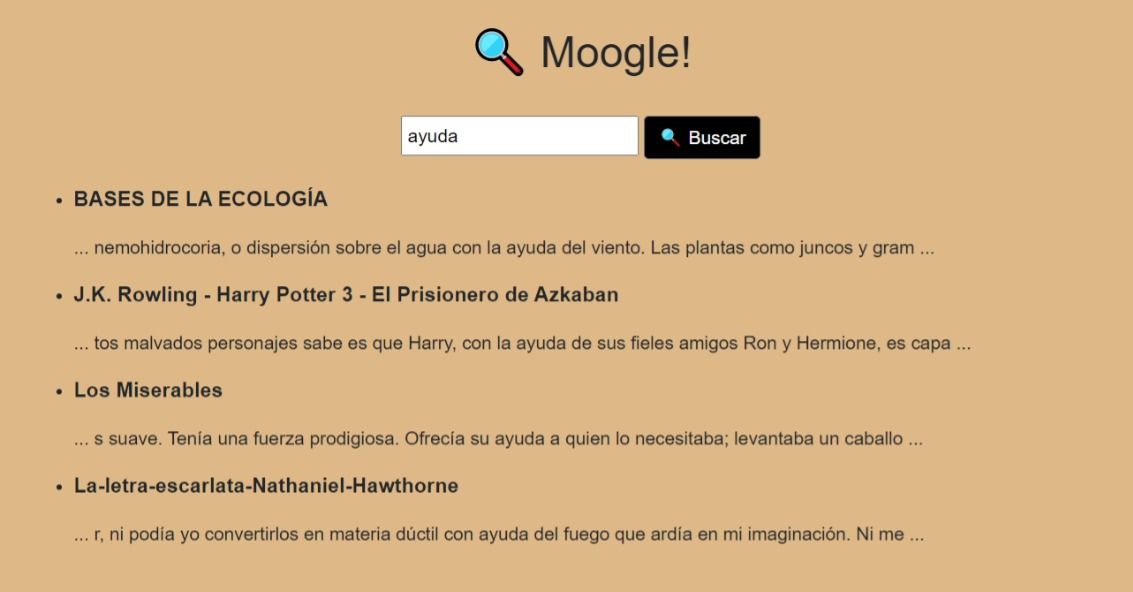
\includegraphics[width=14cm]{Web1.jpg}
       \caption{Ejemplo de búsqueda}
       \label{fig:example}
\end{figure}

\item Fragmentos de Texto:
   Junto a cada resultado, se mostrará un fragmento del texto que corresponde a la búsqueda realizada. Esto le brindará una vista previa del contenido relevante encontrado en cada archivo.

\item Sugerencias de Búsqueda:
   En el caso de que alguna palabra de su consulta no aparezca en ningún archivo de la colección, verá una sugerencia de búsqueda más similar que contenga palabras que sí se encuentren en la colección. Esto le permitirá ajustar su consulta para obtener resultados más precisos.

\begin{figure}[h]
       \center
       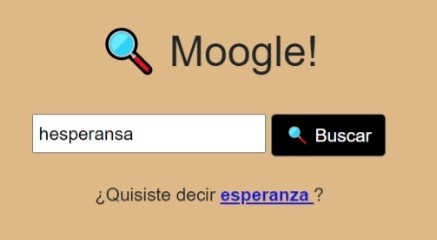
\includegraphics[width=10cm]{Web3.jpg}
       \caption{Ejemplo de sugerencia}
       \label{fig:suggestion}
\end{figure}
\end{enumerate}





\newpage
\section{Bases Conceptuales}\label{sec;base}
En el mundo actual de la información digital, el acceso rápido y preciso a los contenidos es de suma importancia. Con el objetivo de proporcionar una experiencia de búsqueda más efectiva, es que se desarrolla este proyecto de un buscador mejorado que utiliza conceptos como TF-IDF, similitud por coseno y distancia de Levenshtein.

\subsection{TF-IDF}
TF-IDF (Term Frequency-Inverse Document Frequency) es una medida que evalúa la relevancia de una palabra en un documento en relación con una colección de documentos. Utilizamos esta técnica para asignar un peso a cada palabra en un documento y así capturar la importancia relativa de cada término. La fórmula implementada en este proyecto es la siguiente:

\[TF-IDF = \frac{Xi}{Ni} \times ln\left(\frac{D}{P}\right)\]
Donde:
\begin{itemize}
\item $Xi$
representa la frecuencia absoluta de una palabra en un documento.
\item $Ni$
representa la cantidad de palabras del documento en cuestión.
\item $D$
representa la cardinalidad de la colección de documentos.
\item $P$
representa la cantidad de documentos en los que aparece la palabra.
\end{itemize}

En caso de que una palabra no aparezca en ningún documento de la colección , dado que se indefiniría el argumento del logaritmo , mediante una estructura de control de flujo (condicional if) se garantiza que el valor TF-IDF de esa palabra sea 0. Cabe destacar que si la palabra está presente en todos los documentos de la colección entonces su TF-IDF será 0 también puesto que al ser tan común pierde relevancia.

\paragraph{\textcolor{red}{
A cada uno de los documentos le es asignado un vector (un array de double), donde cada componente representa el tf-idf en ese documento de cada palabra presente en toda la colección. Estos vectores son usados para su comparación con la entrada del usuario, a la que también se le asigna un vector de la misma forma.}}


\subsection{Similitud por coseno}
 La similitud por coseno es una medida que se utiliza comúnmente en recuperación de información y análisis de texto para determinar la similitud entre dos vectores de características. Esta técnica es especialmente útil cuando se trata de comparar textos o documentos basados en el contenido y la frecuencia de las palabras.

El procedimiento para calcular la similitud por coseno involucra varios pasos:

\begin{enumerate}
\item Creación de los vectores de los textos a comparar. En este caso se utilizó el cálculo de TF-IDF para su elaboración.
\item Cálculo del producto punto:
\begin{itemize}
 \item  El producto punto se calcula multiplicando las correspondientes componentes de los vectores y sumando los productos. Por ejemplo, el producto punto entre los vectores [2, 1, 0, 3] y [1, 0, 1, 2] sería: \[(2\times 1) + (1\times 0) + (0\times 1) + (3\times 2) = 8\].
\end{itemize}
\item  Cálculo de las magnitudes de los vectores:
\begin{itemize}
  \item  La magnitud de un vector se calcula sumando los cuadrados de sus componentes y luego tomando la raíz cuadrada del resultado.
  \item  Por ejemplo, la magnitud del vector [2, 1, 0, 3] se calcularía como:\[\sqrt{(2^2) + (1^2) + (0^2) + (3^2)} = \sqrt{4 + 1 + 0 + 9} = \sqrt{14}\].
\end{itemize}

\item Cálculo de la similitud por coseno:
\begin{itemize}
   \item Finalmente, la similitud por coseno se calcula dividiendo el producto punto de los vectores por el producto de sus magnitudes.
   \item La fórmula para calcular la similitud por coseno es: \[\text{similitud} = \frac{{\text{producto punto}}}{{\text{magnitud vector1} \times \text{magnitud vector2}}}\].
  \item En el ejemplo anterior, la similitud por coseno entre los vectores [2, 1, 0, 3] y [1, 0, 1, 2] sería: \[\frac{8}{{\sqrt{14} \times \sqrt{6}}} \approx 0.765\].
\end{itemize}
\end{enumerate}
La similitud por coseno proporciona un valor entre 0 y 1, donde 0 indica ninguna similitud y 1 indica una similitud total entre dos vectores de características. Cuanto más cercano esté el valor a 1, mayor será la similitud entre los vectores.

Este procedimiento de cálculo es una representación básica de cómo se calcula la similitud por coseno entre un documento y la entrada del usuario que es utilizada para oraganizarlos de acuerdo a su relevancia (mientras mayor sea la similitud mayor será la relevancia).

\subsection{Distancia de Levenshtein}
La distancia de Levenshtein, también conocida como distancia de edición, es una métrica utilizada para cuantificar la diferencia entre dos cadenas de caracteres. Fue propuesta por Vladimir Levenshtein en 1965 y se utiliza ampliamente en campos como la corrección ortográfica, la bioinformática y la recuperación de información.

La distancia de Levenshtein se calcula determinando el número mínimo de operaciones requeridas para transformar una cadena en otra. Las operaciones permitidas son:
\begin{enumerate}

\item Inserción: Insertar un carácter en una cadena.
\item Eliminación: Eliminar un carácter de una cadena.
\item Sustitución: Reemplazar un carácter de una cadena por otro.
\end{enumerate}
Cada una de estas operaciones tiene un costo unitario asociado. La distancia de Levenshtein es la suma de los costos de todas las operaciones necesarias para transformar una cadena en la otra.

Por ejemplo para transformar 'casa' en 'cala', podemos realizar una sustitución del carácter 's' por 'l'. Esto implica una operación con un costo de 1. Por lo tanto, la distancia de Levenshtein entre estas dos cadenas sería 1.

 Esta medida es implementada con el objetivo de construir una sugerencia al usuario en caso de que al menos una de las palabras de la búsqueda no exista en la colección de documentos. Para ello se selecciona(n) la(s) palabra(s) de menor distancia de Levenshtein con la(s) que no aparece(n) en la colección y se construye una nueva sentencia con la(s) palabra(s) sustituida(s).
El siguiente fragmento de código representa el método utilizado en el proyecto para determinar la distancia de Levenshtein entre dos palabras:
\begin{lstlisting}[language= Java]
public static double DistanciaLevenshtein(string str1, string str2)
    {
        //Calculo de la distancia de Levenshtein
        int longitudStr1 = str1.Length;
        int longitudStr2 = str2.Length;
        int[,] matrizDistancia = new int[longitudStr1 + 1, longitudStr2 + 1];

        if (longitudStr1 == 0)
        {
            return longitudStr2;
        }

        if (longitudStr2 == 0)
        {
            return longitudStr1;
        }

        for (int i = 0; i <= longitudStr1; i++)
        {
            matrizDistancia[i, 0] = i;
        }

        for (int j = 0; j <= longitudStr2; j++)
        {
            matrizDistancia[0, j] = j;
        }

        for (int i = 1; i <= longitudStr1; i++)
        {
            for (int j = 1; j <= longitudStr2; j++)
            {
                int costo = (str2[j - 1] == str1[i - 1]) ? 0 : 1;
                matrizDistancia[i, j] = Math.Min(Math.Min(matrizDistancia[i - 1, j] + 1, matrizDistancia[i, j - 1] + 1), matrizDistancia[i - 1, j - 1] + costo);
            }
        }

        return (double)matrizDistancia[longitudStr1, longitudStr2];
    }
\end{lstlisting}


\newpage
\section{Estructura del proyecto}\label{sec;class}
La aplicación está estructurada en dos partes fundamentales: \textcolor{blue}{Moogle Server} y \textcolor{blue}{Moogle Engine}.

\subsection{Moogle Server}\label{sub;serv}
   \textcolor{blue}{MoogleServer} es un servidor web que renderiza la interfaz gráfica y sirve los resultados. Aquí se modificó parte de la interfaz gráfica en algunos aspectos, algunos triviales como la personalización y otros con el objetivo de favorecer la experiencia del usuario como el poder acceder a la búsqueda sugerida mediante un hipervínculo.

\subsection{Clases de Moogle Engine}\label{sub;engine}
 Se utilizó el modelo vectorial de recuperación de información por las ventajas que ofrece: el esquema de ponderación y la estrategia de coincidencia parcial. Con coincidencia parcial se hace referencia a que la consulta no tiene que coincidir exactamente con un documento para ser considerado relevante. Por ejemplo, un documento relevante puede no cumplir con todos los requerimientos de la consulta sino con un subconjunto de ellos. Son precisamente estas diferencias las que permiten realizar una ordenación de los documentos recuperados. 
 Cada epígrafe de esta subsección  explica a grandes razgos las clases que componen a \textcolor{blue}{Moogle Engine} sobre las que recaen el proceso algebraico del proyecto.

\subsubsection{Clase Coleccion}\label{sub;col}
En la clase \textcolor{orange}{Coleccion} se encuentra todo lo relativo al trabajo con los archivos de la colección de archivos (.txt) que utiliza Moogle como materia prima, de ahí el nombre. Entre sus propiedades más significativas está  \textcolor{red}{TheMatrix} , una matriz, que utilizando :un diccionario \textcolor{red}{Dictionary\textless string, int\textgreater} que asocia a cada palabra presente en el documento su frecuencia en el mismo, una lista \textcolor{red}{List\textless string\textgreater} que contiene las palabras únicas de toda la colección y por supuesto la cardinalidad del conjunto de archivos, implementa los conceptos de TF- IDF para la posterior respuesta a la interacción con el usuario. En esta clase se encuentra también el método  \textcolor{magenta}{VectQuerys}, que sobre la misma base conceptual devuelve el vector TF-IDF de la cadena introducida por el usuario .La clase descansa en la clase  \textcolor{orange}{Metodos}, aquí se encuentra cada una de las funcionalidades más generales que demandan las otras clases, una de ellas es el método  \textcolor{magenta}{Similitud} , que utiliza el procedimiento de similitud por coseno para devolver un array de double que contiene de forma ordenada la puntuación de cada documento de acuerdo a su parecido con el query  (entrada del usuario al programa), esta puntuación va de 0 a 1 y mientras mayor sea, mayor será la similitud y por ende la relevancia del documento para ser devuelto. Lo más interesante de la clase es quizás el método  \textcolor{magenta}{ObtenerSearchItems}, que además de organizar los documentos por su relevancia llamando a métodos de la clase  \textcolor{orange}{Metodos}, como \textcolor{magenta}{MejoresTitulo}, y devolver un array de este tipo de objeto, incorpora a estos un fragmento del documento donde aparece al menos una palabra de la cadena introducida por el usuario, precisamente la de mayor relevancia por su valor de TF-IDF de acuerdo a su aparición en el query, para esto se implementan métodos de la propia clase y otros de la clase  \textcolor{orange}{Metodos} , con el objetivo de organizar el query de acuerdo al TF-IDF de las palabras y especialmente el método  \textcolor{magenta}{Snipet} que busca la primera aparición de la palabra seleccionada en el texto y nos devuelve una vecindad de la misma en  \textcolor{red}{string}.

Este es el código del método  \textcolor{magenta}{ObtenerSearchItems}:
\begin{lstlisting}[language=Java]
public SearchItem[] ObtenerSearchItems(string query)
    {
        //Metodo para retornar el Array con los SearchItems que se ofreceran al usuario
        Query objetoQuery = new Query(query);
        double[] vectorScore = Metodos.Similitud(TheMatrix,VectorQuerys(query, Archivos.Length));
        int[] indicesDeTextos = Enumerable.Range(0, vectorScore.Length).ToArray();
        string[] mejoresTitulos = Metodos.MejoresTitulo(Metodos.CrearDiccionario(Titulos,vectorScore));
        Array.Sort(vectorScore,indicesDeTextos);

        Array.Reverse(indicesDeTextos);

        Array.Reverse(vectorScore);
        
        List<SearchItem> searchItems = new List<SearchItem>();
        //Ordenar el query de acuerdo a la relevancia de cada una de sus palabras
        string[] terminosQuery = OrdenarQuery(objetoQuery.TerminosQuery, VectorQuerys(query,Archivos.Length));
     
        for (int i = 0; i < vectorScore.Length; i++)
        {
            //solo se devolvera aquellos searchitems cuyo score es mayor que cerp
            if (vectorScore[i] > 0)
            {
                string snippet = "";
                if(ListaPalabrasSinRep.Contains(terminosQuery[0]))
                {
                 snippet = Metodos.Snipet(terminosQuery[0],Archivos[indicesDeTextos[i]]);
                }
                else if(ListaPalabrasSinRep.Contains(terminosQuery[1]))
                {
                 snippet = Metodos.Snipet(terminosQuery[1],Archivos[indicesDeTextos[i]]);   
                }
                else
                {
                  snippet = Metodos.Snipet(terminosQuery[2],Archivos[indicesDeTextos[i]]);   
                }
                searchItems.Add(new SearchItem(mejoresTitulos[i],snippet,(float)vectorScore[i]));
            }
            else break;
        }
      return searchItems.ToArray();
    }

\end{lstlisting}


\paragraph{\textcolor{blue}{Sugerencia} }\label{sub:center}
En esta clase además se encuentran los métodos necesarios para la salida de la sugerencia. Si en la cadena introducida por el usuario no aparece al menos una de las palabras en toda la colección entonces aparecerá en la pantalla una sugerencia que será la propia entrada con la palabra que no aparece cambiada por la palabra de la colección de menor Distancia de Levenshtein con ella, para determinar esta distancia se implementa el método \textcolor{magenta}{DistanciaLevenshtein} de la clase \textcolor{orange}{Metodos}, y los métodos que se encuentran al final de la clase Coleccion determinan la necesidad de sugerencia y la construyen cuando es llamado el método  \textcolor{magenta}{Sugerencia} , desde la clase \textcolor{orange}{Moogle}. 
\begin{lstlisting}[language=Java]
public string Sugerencia( string query)
    {
        //Este Metodo es el que retorna la sugerencia final implementando todos los anteriores y es llamado desde Moogle
        Query objetoQuery = new Query(query);
        string[] palabras = objetoQuery.TerminosQuery;
        if(NecesidadSugerencia(palabras))
        {
          return ConstructorSugerencia(query); 
        }
        else
        return "";
    }
\end{lstlisting}

\subsubsection{Clase Query}\label{sub;query}
La clase \textcolor{orange}{Query} es la más simple , su única propiedad es un array de string que contiene como términos a las palabras de la query, de ahí que para crear un objeto de este tipo es necesario pasarle como argumento un string que es precisamente la entrada del usuario.
\begin{lstlisting}[language=Java]
namespace MoogleEngine;

public class Query
{
    public string[] TerminosQuery;
    public Query(string query)
    {
        TerminosQuery = Metodos.SepararPalabras(query);
    }
}
\end{lstlisting}


\subsubsection{Clase Metodos}\label{sub;meth}
La clase es asistencial, solamente contiene métodos para ser usados en la clase \textcolor{orange}{Coleccion}, encargados de leer los archivos y asistir a otros métodos.  Algunos de estos métodos son los siguientes:
\begin{itemize}

\item Este método calcula la magnitud de cada vector usada para calcular la similitud por coseno: 
\begin{lstlisting}[language=Java]
 public static double Norma(double[] a)
    {
        //Este Metodo Calcula la norma de cada vector
        double suma = 0;
        for (int i = 0; i < a.Length; i++)
        {
            suma += Math.Pow(a[i], 2);
        }
        double norma = (Math.Sqrt(suma));
        return norma;
    }
\end{lstlisting}

\item Este método devuelve los titulos de los documentos más relevantes organizados:
\begin{lstlisting}[language=Java]
 public static string[] MejoresTitulo(Dictionary<string, double> diccionario)
    {
        //Organiza los titutlos de acuerdo a su score
        string[] mejoresTitulos = new string[diccionario.Count];
        int count = 0;
        foreach (var item in diccionario.OrderByDescending(item => item.Value))
        {
            mejoresTitulos[count] = item.Key;
            count++;
        }
        return mejoresTitulos;
    }
\end{lstlisting}

\item Este método calcula la similitud por coseno:
\begin{lstlisting}[language=Java]
public static double[] Similitud(double[,] matriz, double[] vectorQuery)
    {
        double[,] TheMatrix = matriz;
        //ahora vamos a determinar la similitud por coseno
        //primero calculamos el producto  punto de los vectores de la matriz y el vector del query
        double[] ProductoPunto = MatrizPorVector(TheMatrix, vectorQuery);
        //despues calculamos la norma de cada vector
        double[] Normas = new double[ProductoPunto.Length];
        double normaVector = Norma(vectorQuery);
        for (int i = 0; i < Normas.Length; i++)
        {
            double[] temp = new double[TheMatrix.GetLength(1)];
            for (int j = 0; j < temp.Length; j++)
            {
                temp[j] = TheMatrix[i, j];
            }
            Normas[i] = Norma(temp);
        }
        //Ahora debemos calcular el producto de las normas de los  vectores 
        for (int i = 0; i < Normas.Length; i++)
        {
            Normas[i] *= normaVector;
        }
        //Ahora debemos dividir el producto punto de los vectores entre el producto de sus normas
        double[] score = new double[ProductoPunto.Length];
        for (int i = 0; i < ProductoPunto.Length; i++)
        {
            if (Normas[i] != 0)
                score[i] = ProductoPunto[i] / (double)Normas[i];
            else
                score[i] = 0;
        }
        return score;
    }
\end{lstlisting}
\end{itemize}



\subsubsection{Clase Moogle}\label{sub;moog}
La clase \textcolor{orange}{Moogle} contiene un método void que inicializa al objeto de tipo \textcolor{red}{Coleccion} coleccion, y dentro de su método \textcolor{magenta}{Query} de tipo \textcolor{red}{SearchResult} llama a los métodos de la clase \textcolor{orange}{Coleccion} , \textcolor{magenta}{ObtenerSearchItems} y
 \textcolor{magenta}{Sugerencia} para devolver el objeto \textcolor{red}{SearchResult}.
\begin{lstlisting}[language=Java]

namespace MoogleEngine;
public static class Moogle
{
//Creacion objeto de tipo Coleccion
    public static Coleccion coleccion;
    public static SearchResult Query(string query) 
    {
        SearchItem[] searchItem = coleccion.ObtenerSearchItems(query);
        string sugerencia = coleccion.Sugerencia(query);
        return new SearchResult(searchItem, sugerencia);
    }

    public static void Iniciar()
    {
        coleccion = new Coleccion();
    }
}
\end{lstlisting}
            


\newpage

\section{Conclusiones}\label{sec:concl}
La creación de este proyecto ha sido sumamente instructiva sobre temas como encapsulamiento y Álgebra Lineal y ha contribuido sólidamente a fortalecer habilidades como la investigación y otras menos interactivas pero igualmente importantes como son la organización y la planificación, tan necesarias para la vida profesional.
\end{document}












































